% !TEX root = ../gnss_interference_resistant_thesis.tex
\documentclass[main.tex]{subfiles}

\begin{document}

\subsection{Spindulio formavimo rezultatai}\label{sec:beam_form_results}

Matavimai atliekami \ref{sec:beamform_meas_stand} skyriuje aprašytame stende,
su 2 spinduolių sistema, pirmas matavimas atliekamas su viena
antena, antrasis - su dviem antenomis esant 0 fazės skirtumui ir trečias matavimas - su dviem
spinduoliais ir esant $2\ \mathrm{rad}$ fazės skirtumui. Antenos yra išdėstytos $\lambda / 2$ atstumu,
todėl esant $2\ \mathrm{rad}$ fazės skirtumui, tikimasi, kad diagramos maksimumas bus nukreiptas 40 laipsnių
kampu.

\begin{figure}[h]
    \begin{centering}
    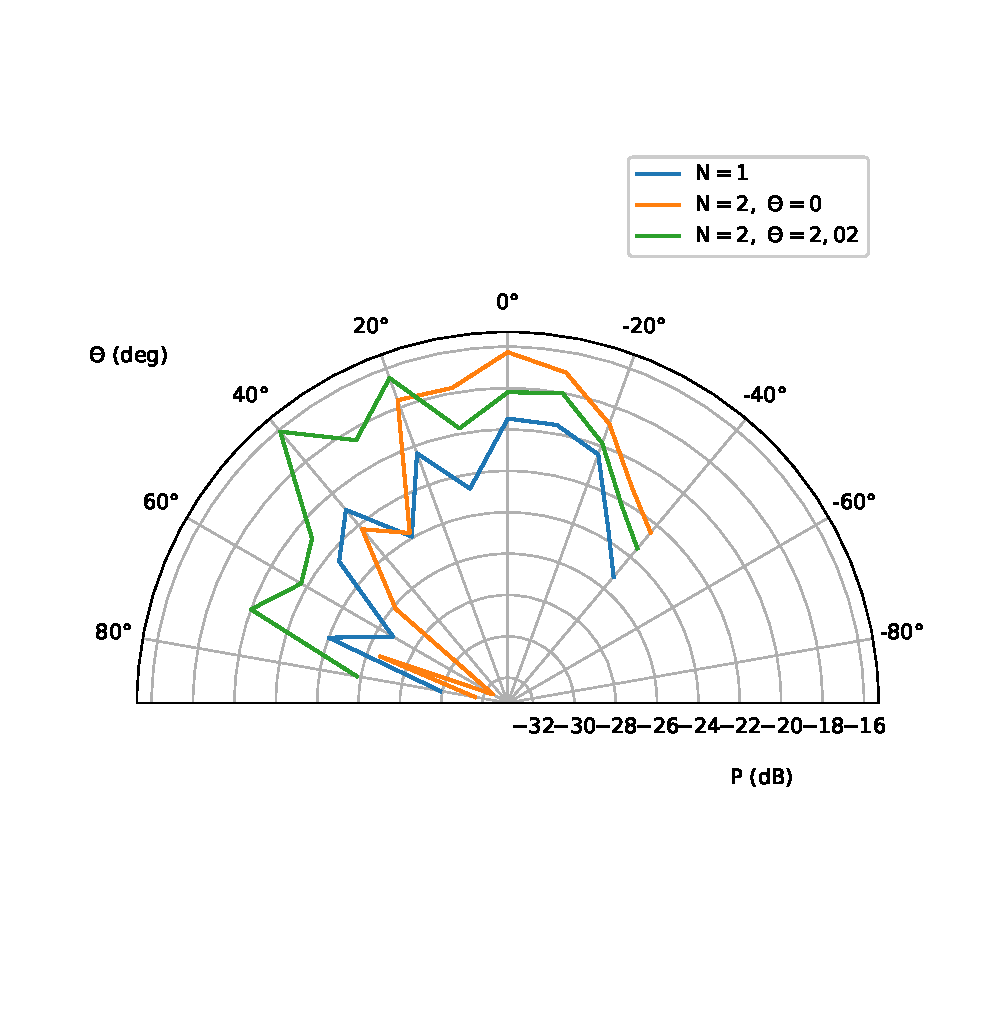
\includegraphics[scale=0.8]{drawings/beam_forming_results}
    \par\end{centering}
    \protect\caption{\label{fig:beamforming_result}Antenų sistemos spinduliavimo diagramos esant skirtingam spinduolių skaičiui
    ir skirtingai fazei tarp spinduolių.}
\end{figure}

Iš \ref{fig:beamforming_result}~pav. galima nustatyti, kad naudojant viena spinduolį, diagramos maksimumas
yra $-19,4\ \mathrm{dB}$ ir yra nukreiptas 0 laipsnių kampu. Įjungus antrą anteną iškarto stebimas
$3\ \mathrm{dB}$ maksimumo padidėjimas iki $-16,4\ \mathrm{dB}$. Toks signalo padidėjimas reiškia,
kad priimama galia padidėjo 2 kartus, kadangi signalas priimamas iš dviejų antenų.

Vienam iš imtuvų pritaikius $\Delta \Theta = 2\ \mathrm{rad}$ fazės pokytį, gauta, kad
maksimumas pasislinko į 40 laipsnių kryptį, o signalo stiprumas išliko toks pat kaip atveju
kai fazės pokyčio
nebuvo. Šis rezultatas sutampa su \refeq{eq:phase_shift_antenna_angle} lygties rezultatu.

Visi matavimų grafikai turi tam tikrus minimumus, ten kur jų neturėtų būti. Jie atsiranda
dėl stovinčių bangų, kadangi matavimai buvo atlikti patalpoje nuo kurios sienų vyksta
atspindžiai. Norint gauti tikslines spinduliavimo diagramas, matavimus reiktų
atlikti patalpoje, kurioje nėra atspindžių.

Iš gautų rezultatų galime daryti išvada, kad naudojant HackRF imtuvus spindulio formavimas
yra galimas, gaunamas $3\ \mathrm{dB}$ signalo sustiprėjimas ir pritaikius fazės pokytį,
galima keisti spinduolių sistemos kryptingumo diagramą.


\end{document}
